
\chapter{Package implementation in R}
\label{cha:R}

Once understood what Bitcoin Cash is, how the technology works behind it and the
reasons why it was created. We are going to describe how we can extract information
from the blockchain using the R programming environment. We will describe how we
can read blocks and all the data inside them, allowing us to make some useful analysis
on the Bitcoin Cash behaviour. 

\section{R}
\label{sec:environment}

R\cite{rint} is an Open Source software for statistical computing (linear and nonlinear
 modeling, classical statistical tests, time-series analysis, classification,
 clustering) and graphics. One of R’s strengths is the ease with which well-designed 
 publication-quality plots can be produced, including mathematical symbols and 
 formulae where needed.\\
R is designed around a true computer language, and it allows users to add additional 
functionality by defining new functions. Much of the system is itself written in the 
R which makes it easy for users to follow the algorithmic choices made. But, for
computationally-intensive tasks, C, C++ and Fortran code can be linked and called 
at run time. Furthermore, thanks to its Open Source nature, it can be easily extended
via "Packages" even written by the user.\cite{rint}

\section{Feasibility study}
\label{sec:study}

The goal for this project is to extend the R language with a package which allows us
to read and analyse the information contained into the Bitcoin Cash blockchain.\\
To make it in the best way, firstly, a research for the existing implementations has 
been done, but unfortunately, without any result. Except for two 
completely different ways to build the package. \\
The first one was to turn the used device into a node of the Bitcoin Cash network.
This lead the user to download all the blockchain and make all the queries locally.
As a result, the queries turned out to be very fast and all the data of the blockchain 
manipulated as one may desire. But, on the other hand, storing all the blockchain 
requires a lot of space on the device (around 143 GigaByte on 13/9/2019). So making
a package of that size does not seem to be the best option.\\
For these reasons, the second way was chosen. Although it is the slowest implementation,
it avoided the need to become a node of the network, and thus making the installation of the
package very simple and fast. That was obtained by relying on a service provider (SP).

\section{Package integration}
\label{sec:integration}

For the second option, it was rather difficult to find a SP which 
not only implemented an "Application Programming Interface" (API)\cite{api} where one could
make queries and have the wanted data as a response. But also made it public, 
so anyone can use it. Additionally, the service providers were chosen also 
according to the amount of data provided, the format of the response and the 
number of queries one was allowed to make. At the end, the picks were:
\begin{itemize}
    \item Blockdozer Explorer.
    \item Blockchair.
\end{itemize} 
The motivation for these two options was the fact that they were complementary.
The first one allowed an unlimited number of queries returning essential information.
The second one instead, had a limit of 30 queries per minute but returned more 
and better-formatted data. 

Let us begin with the technical implementation by saying that in order to maintain all the R project, 
was used the RStudio editor\cite{rstudio} has been used.\\ 
First of all, it is necessary to create and manage a new package in R. For this 
purpose, some other packages are required : 
\begin{itemize}
    \item \textit{devetools}   : to manage the project and the source code of the new package.
    \item \textit{roxygenize2} : to handle all the documentation of the package.
\end{itemize}
Then it is necessary to install the other two packages to handle the data and the connection with 
the service providers.
\begin{itemize}
    \item \textit{httr}        :to perform correctly the Http requests to the service providers and receive the linked response
    \item \textit{jsonlite}    :to manipulate and store the received data, in order to have a good dataset for the future analysis
\end{itemize}
With these tools is possible to proceed to the performing of a simple query to an API. Suppose one might to know
some information about a specific Bitcoin Cash address. After choosing the appropriate SP,
their documentation must be readed and seen how to correctly build the Http request. 
In this case, the pattern is: \medskip

\textit{GET /api/addr/\{paymentAddress\}[?noTxList\&from\&to\&returnLegacyAddresses]}
\\
\begin{figure}[h]
    \centering
    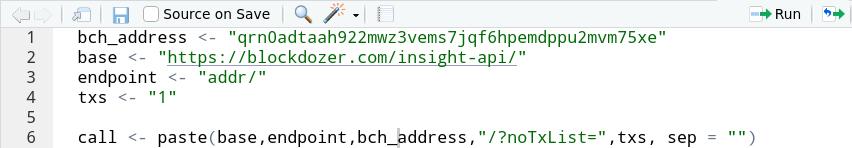
\includegraphics[height=2cm]{create_call.png}
    \caption{Example of the building of an Http request}
    \label{fig:request}
\end{figure}\\
With a few lines code, we can then construct a possible request for the desired information. 
As a result one can have:\medskip

\textit{https://blockdozer.com/insight-api/addr/qrn0adtaah922mwz3vems7jqf6hpemdppu2mvm75xe/?noTxList=1}
\medskip\\
As said before, the response will be in a \textit{json} format and will be handled thanks to the
\textit{jsonlite} package. But due to the multiple ways to manipulate the data, it is 
suggested to look the source code on the GitHub repository: \url{github.com/PopBogdan97/bCashReader}
\begin{figure}[h]

    \centering
    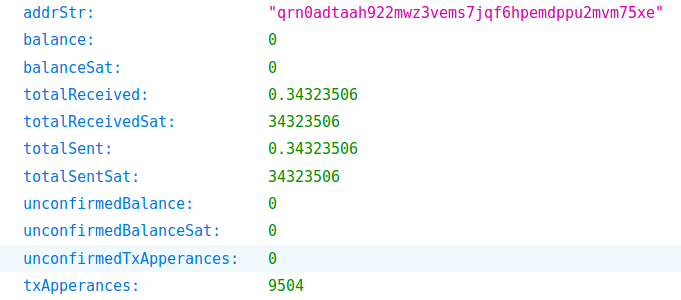
\includegraphics[height=5cm]{json_sample.png}
    \caption{Example \textit{json} response}
    \label{fig:response}
\end{figure}\pagebreak


\subsection{Commands}
\label{sec:commands}

Due to the multiple data formats provided by the Service Providers and the 
different information that can be retrieved from the Bitcoin Cash blockchain, 
one can subdivide all the implemented commands in four macro categories.\medskip\\
\textbf{Address Commands.} All the next commands give the possibility to make different
type of queries on the address details by giving only address identifier as the argument
of the function. It could be in both LegacyAddress (those similar to Bitcoin) and Cashaddr
(the new format eplained here \ref{sec:addresses}).
\begin{table}[!ht]
    \centering
    \begin{tabular}{||l|p{6cm}||}
    \hline
    \textbf{Function}                          & \textbf{Description}                                                  \\ \hline
    \textit{addr\_balance(hash string)}                 & Get the balance of a Bitcoin Cash address.                            \\ \hline
    \textit{addr\_history(hash string)}                 & Get the general data (history) of a Bitcoin Cash address.             \\ \hline
    \textit{addr\_totalReceived(hash string)}           & Get the total amount of Bitcoin Cash received by the address.         \\ \hline
    \textit{addr\_totalSent(hash string)}               & Get the total amount of Bitcoin Cash sent by the address.             \\ \hline
    \textit{addr\_txApperances(hash string)}            & Get the total amount of transactions made by the address.             \\ \hline
    \textit{addr\_txs(hash string)}                     & Get the all the transactions made by the address.                     \\ \hline
    \textit{addr\_unconfirmedBalance(hash string)}      & Get the unconfirmed balance of a Bitcoin Cash address.                \\ \hline
    \textit{addr\_unconfirmedTransactions(hash string)} & Get the total amount of unconfirmed transactions made by the address. \\ \hline
    \textit{addr\_utxo(hash string)}                    & Get the unspent transactions (UTXO) of an address.                    \\ \hline
    \end{tabular}
    \end{table}\\
\textbf{Block Commands.} The underlying commands allow to retrieve all the information about the 
blocks by inserting as parameter of the function three types data: \textit{Date, block's hash}, and \textit{block's height }in the blockchain.
\begin{table}[!ht]
    \centering
    \begin{tabular}{||l|p{6cm}||}
    \hline
    \textbf{Function}                          & \textbf{Description}                                                  \\ \hline
    \textit{block\_byDate("yyyy-MM-dd" string)}                 & Get all the blocks in a specific Date with the format yyyy-MM-dd.                          \\ \hline
    \textit{block\_byDateCount("yyyy-MM-dd" string)}    & Get the block count in a specific Date with the format yyyy-MM-dd.             \\ \hline
    \textit{block\_byHash(hash string)}                 & Get the information of a specific Bitcoin Cash block (without the transactions).         \\ \hline
    \textit{block\_byHashRaw(hash string)}              & Get the raw information of a specific Bitcoin Cash block.             \\ \hline
    \textit{block\_byHashTxs(hash string)}              & Get the transaction hashes of a specific Bitcoin Cash block.             \\ \hline
    \textit{block\_byHeight(height integer)}            & Get the information contained in a specific Bitcoin Cash block.                     \\ \hline
    \end{tabular}
    \end{table}\pagebreak\\
\textbf{Transaction Commands.} The later functions return the information of a specific transaction and its 
inputs and outputs by knowing the \textit{transaction hash}.
\begin{table}[!ht]
    \centering
    \begin{tabular}{||p{6.2cm}|p{6cm}||}
    \hline
    \textbf{Function}                          & \textbf{Description}                                                  \\ \hline
    \textit{txs\_byHash(hash string)}                   & Get the all the information of a specific transaction.                          \\ \hline
    \textit{txs\_byHashIn(hash string)}         & Get the all the information of a specific transaction inputs.      \\ \hline
    \textit{txs\_byHashOut(hash string)}                & Get the all the information of a specific transaction outputs.          \\ \hline
    \end{tabular}
    \end{table}\\
To see the description of the alle values retrieved by the functions visit the Blockchair 
documentation\cite{blockchair} in section \textit{Dashboard/transaction}\medskip \\
\textbf{Chain Commands.} These last commands give live information and statistics on the behaviour of the Bitcoin Cash 
blockchain.
\begin{table}[!ht]
    \centering
    \begin{tabular}{||p{6.2cm}|p{6cm}||}
    \hline
    \textbf{Function}                          & \textbf{Description}                                                  \\ \hline
    \textit{chain\_currency()}                           & Get the Bitcoin Cash current value..                          \\ \hline
    \textit{chain\_stats()}                              & Get the Bitcoin Cash current blockchain stats.              \\ \hline
   \end{tabular}
    \end{table}\\
    To see the description of the alle values retrieved by the functions visit the Blockchair documentation\cite{blockchair} in section \textit{Dashboard/stats}\newpage


